    \documentclass[12pt,a4paper]{article}
    \usepackage[T2A]{fontenc}
    \usepackage[utf8]{inputenc}
    \usepackage[russian]{babel}
    \usepackage{amsmath}
    \usepackage{amssymb}
    \usepackage{graphicx}
    \usepackage{floatrow}
    \usepackage{booktabs}
    \usepackage{wrapfig}
    \usepackage{lipsum}
    \usepackage{subcaption}
    \usepackage{fancyhdr}
    \usepackage{mathrsfs}
    \usepackage{tikz}

    \usepackage{graphicx, scalerel}
    \usepackage[warn]{mathtext}
    \usepackage{indentfirst}
    \usepackage[margin = 25mm]{geometry}
    \usepackage{caption}
    \usepackage{multirow}
    \usepackage{gensymb}
    
    \newcommand{\figref}[1]{(См. рис. \ref{#1})}
    \newcommand{\secref}[1]{(См. раздел. \ref{#1})}
    
    \newcommand{\e}[1]{\text{$\cdot10^{#1}$}}
    
    \pagestyle{fancy}
    \fancyhead{}
    \fancyhead[L]{Работа 5.1.2}
    \fancyhead[R]{}
    \fancyfoot[C]{\thepage}
    
    \author{\normalsize Выполнил: Голубович Тимур, группа Б01-110 \\
    	\normalsize 01.11.2023}
    \date{}

    \usepackage{float}
    \restylefloat{table}
    \title{
    	\large Отчет о выполнении лабораторной работы 5.1.2 \\
    	\Large Исследование эффекта Комптона
     }

    \begin{document}
    	\maketitle

    \section*{Цель работы}

    С помощью сцинтилляционного спектрометра исследовать энергетический спектр $\gamma$-квантов, рассеянных на графите. Определить энергию рассеянных $\gamma$-квантов в зависимости от угла рассеяния, а также энергию покоя частиц, на которых происходит комптоновское рассеяние.


    \section*{Оборудование и приборы}

    Источник  $\gamma$-квантов со свинцовым коллиматором; набор поглотителей из различных материалов; сцинтилляционныйй счётчик; пересчётный прибор.
	
    \section*{Теоретическое введение}

    Рассеяние $\gamma$-лучей в веществе относится к числу явлений, в которых особенно ясно проявляется двойственная природа излучения. Волновая теория, хорошо объясняющая рассеяние длинноволнового излучения, испытывает трудности при описании рассеяния рентгеновских и $\gamma$-лучей. Эта теория, в частности, не может объяснить, почему в составе рассеянного излучения, измеренного Комптоном, кроме исходной волны с частотой $\omega_0$ появляется дополнительная длинноволновая компонента, отсутствующая в спектре первичного излучения.
	
	Появление этой компоненты легко объяснимо, если считать, что $\gamma$-излучение представляет собой поток квантов (фотонов), имеющих энергию $\hbar \omega$ и импульс $p = \hbar \omega / c$. Эффект Комптона — увеличение длины волны рассеянного излучения по сравнению с падающим -- интерпретируется как результат упругого соударения двух частиц: $\gamma$-кванта (фотона) и свободного электрона.
	
	Нетрудно получить, что изменение длины волны рассеянного излучения равно
	\begin{equation}
		\Delta \lambda = \lambda_1 - \lambda_0 = \Lambda_\text{к} (1 - \cos\theta),
		\label{Main_Compton}
	\end{equation}
	\noindent где $\lambda_0$ и $\lambda_1$ -- длины волн $\gamma$-кванта до и после рассеяния, а величина
	
	\begin{equation*}
		\Lambda_\text{к} = \frac{h}{mc} = 2.42 \cdot 10^{-10} \text{ см}
	\end{equation*}
	называется комптоновской длиной волны электрона.
 
 
 	Кроме рассеяния $\gamma$-кванты испытывают в среде поглощение, вызываемое фотоэффектом и рождением электрон позитронных пар. Процесс рождения пар пороговый, он возможен лишь при энергии $\gamma$-квантов больше $2mc^2 = 1.02$ МэВ и в рассматриваемом энергетическом диапазоне не происходит. При фотоэффекте из атома выбивается электрон, а квант поглощается. Импульс кванта делится между вылетевшим электроном и атомом, а его энергия частично передается электрону, а частично тратится на возбуждение атома. Атом практически мгновенно (за время порядка $10^{-8}$ с) возвращается в нормальное состояние. Его энергия возбуждения либо излучается в виде мягкого фотона, либо передается какому-нибудь другому электрону, который покидает атом (Оже-эффект). И в том, и в другом случае энергия возбуждения обычно поглощается соседними атомами рассеивателя. Основной целью данной работы является проверка соотношения \eqref{Main_Compton}. Применительно к условиям нашего опыта формулу \eqref{Main_Compton} следует преобразовать от длин волн к энергии $\gamma$-квантов. Как нетрудно показать, соответствующее выражение имеет вид
 	\begin{equation}
 		\frac{1}{\varepsilon(\theta)} - \frac{1}{\varepsilon(0)} = 1 - \cos\theta.
 		\label{Energy_Compton}
 	\end{equation}
 
 	Здесь $\varepsilon(0) = \dfrac{E_0}{mc^2}$ -- выраженная в единицах $mc^2$ энергия $\gamma$-квантов, падающих на рассеиватель, $\varepsilon(\theta)$ -- выраженная в тех же единицах энергия квантов, испытавших комптоновское рассеяние на угол $\theta$, а $m$ -- масса электрона.
 	
 
	\section*{Экспериментальная установка}
	
	Блок-схема установки изображена на рис. \ref{Scheme_Compton}. Источником излучения 1 служит $^{137}$Cs, испускающий $\gamma$-лучи с энергией 662 кэВ. Он помещен в толстостенный свинцовый контейнер с коллиматором. Сформированный коллиматором узкий пучок $\gamma$-квантов попадает на графитовую мишень 2 (цилиндр диаметром 40 мм и высотой 100 мм).
 	
 	\begin{figure}[h!]
 		\centering
 		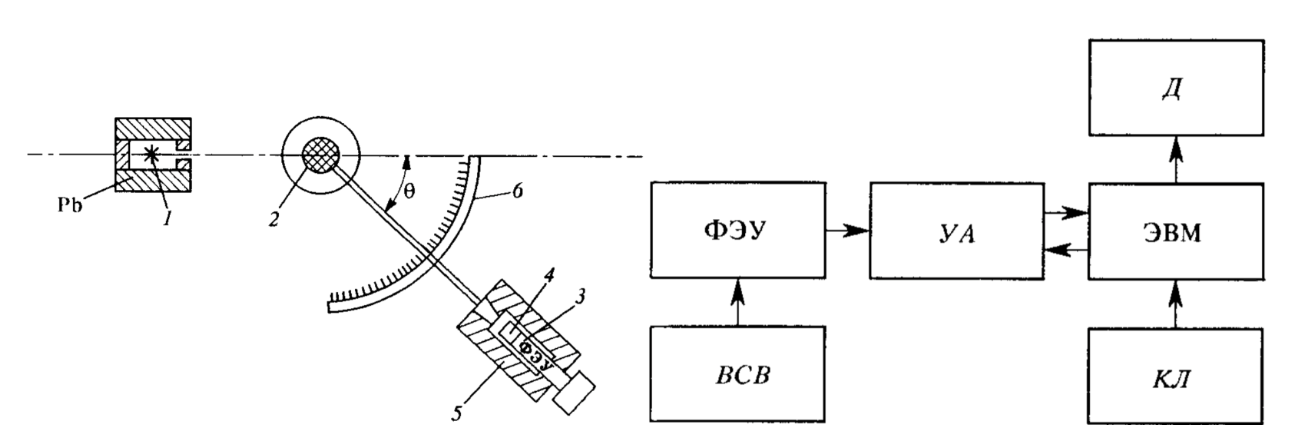
\includegraphics[width=\linewidth]{res/scheme.png}
 		\caption{Экспериментальная установка}
 		\label{Scheme_Compton}
 	\end{figure}
 
 	Кванты, испытавшие комптоновское рассеяние в мишени, регистрируются сцинтилляционным счетчиком. Счетчик состоит из фотоэлектронного умножителя 3 (далее ФЭУ) и сцинтиллятора 4. Сцинтиллятором служит
 	кристалл NaI(Tl) цилиндрической формы диаметром 40 мм и высотой 40 мм, его выходное окно находится в оптическом контакте с фотокатодом ФЭУ. Сигналы, возникающие на аноде ФЭУ, подаются на ЭВМ для амплитудного анализа. Кристалл и ФЭУ расположены в светонепроницаемом блоке, укрепленном на горизонтальной штанге. Штанга вместе с этим блоком может вращаться относительно мишени, угол поворота отсчитывается по лимбу 6.
 	
 	Головная часть сцинтилляционного блока закрыта свинцовым коллиматором 5, который формирует входной пучок и защищает детектор от постороннего излучения. Основной вклад в это излучение вносят $\gamma$-кванты, проходящие из источника 1 через 6-сантиметровые стенки защитного контейнера. Этот фон особенно заметен при исследовании комптоновского рассеяния на большие углы ($\simeq 120^\circ$), когда расстояние между детектором и источником уменьшается.
 	
 	
 	Под действием монохроматического излучения на выходе ФЭУ возникает распределение электрических импульсов. В амплитудном распределении импульсов имеется так называемый фотопик, возникающий в результате фотоэффекта, и обязанное комптоновскому рассеянию сплошное распределение. Часто фотопик называется также пиком полного поглощения, его положение однозначно связана с энергией регистрируемого $\gamma$-излучения.Нас будет интересовать положение (номер канала) вершины этого пика в зависимости от угла поворота детектора.

 
    \section*{Ход работы}

    \begin{enumerate}
		\item Включим все измерительные устройства и компьютер.
		
		\item Запустим программу и войдем в режим измерения спектра.
		
		\item Устанавливая сцинтилляционный счетчик под разными углами $\theta$ к первоначальному направлению полета $\gamma$-квантов и вводя значения этих углов в ЭВМ, снимем амплитудные спектры и определим положения фотопиков для каждого значения угла $\theta$; измерения проведем с шагом $10^\circ$ в диапазоне от $0^\circ$ до $120^\circ$. Результаты запишем в таблицу \ref{Compton_Table}.
	\end{enumerate}
	
	\begin{figure}[h]
		\begin{minipage}[h]{0.49\linewidth}
			\center{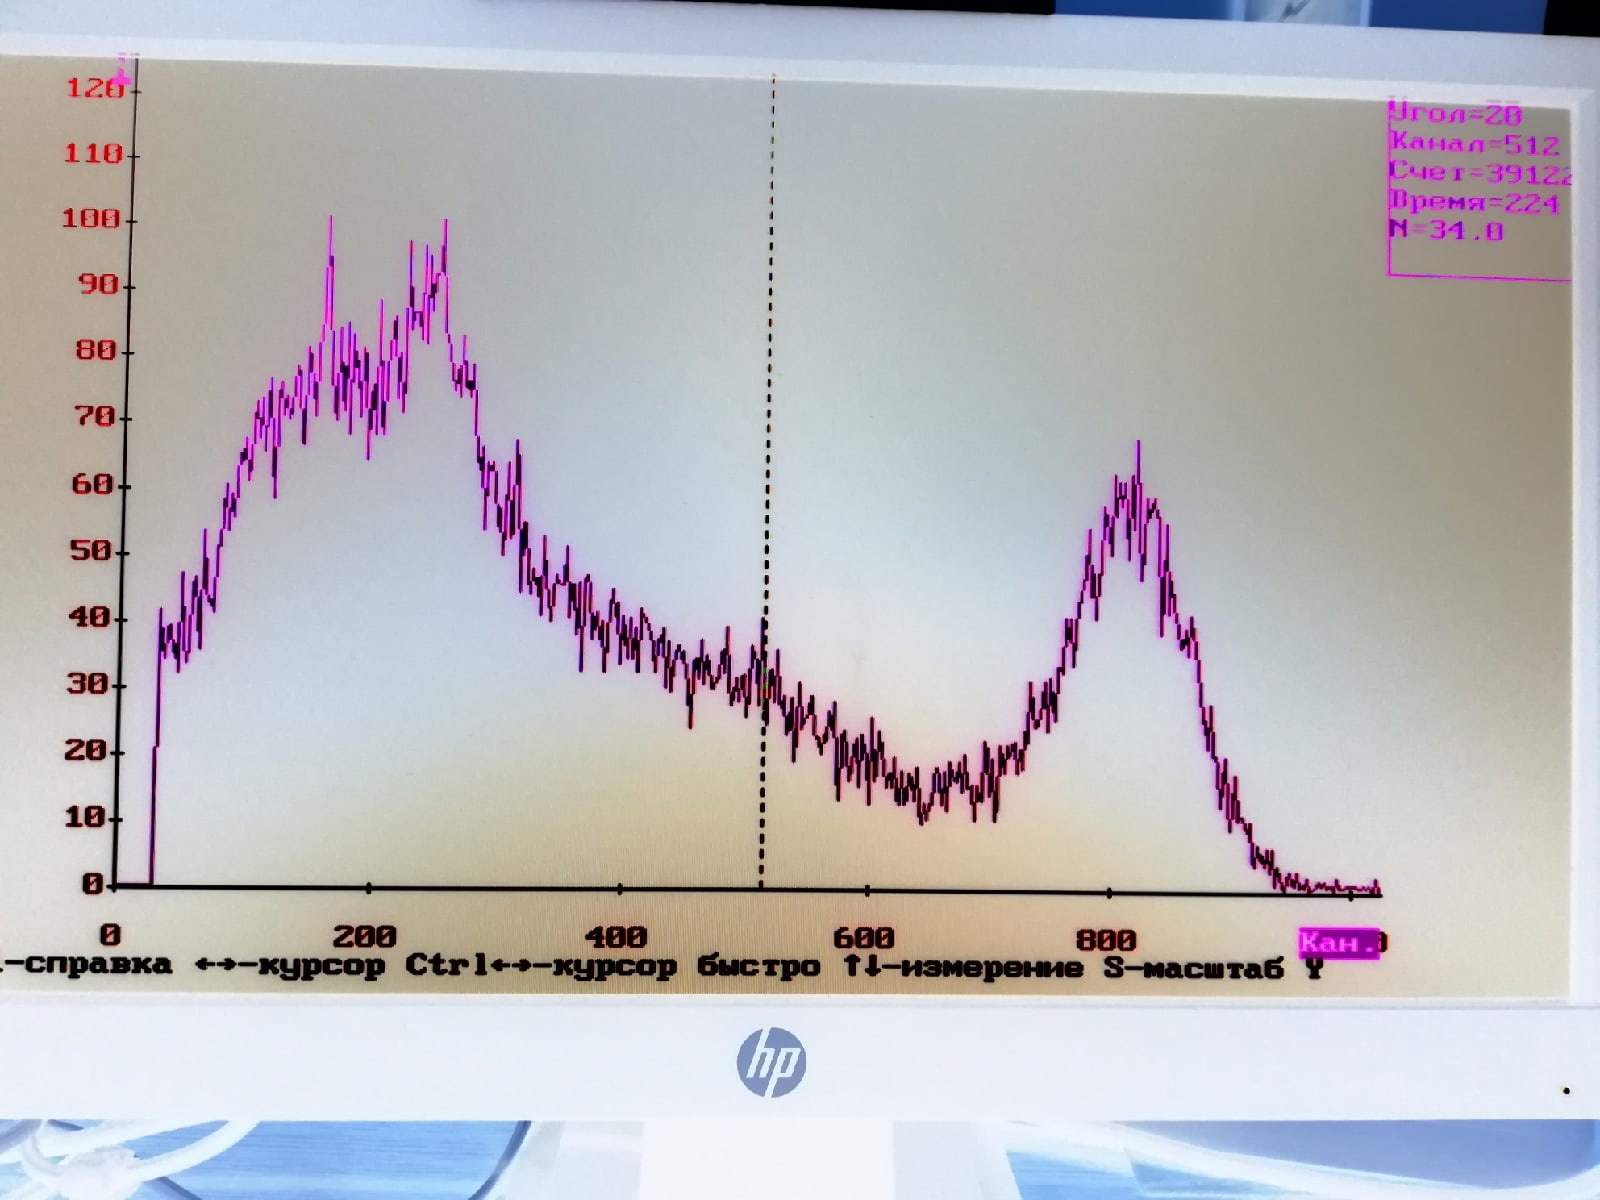
\includegraphics[width=\linewidth]{src/20Neg} \\ а)}
		\end{minipage}
		\hfill
		\begin{minipage}[h]{0.49\linewidth}
			\center{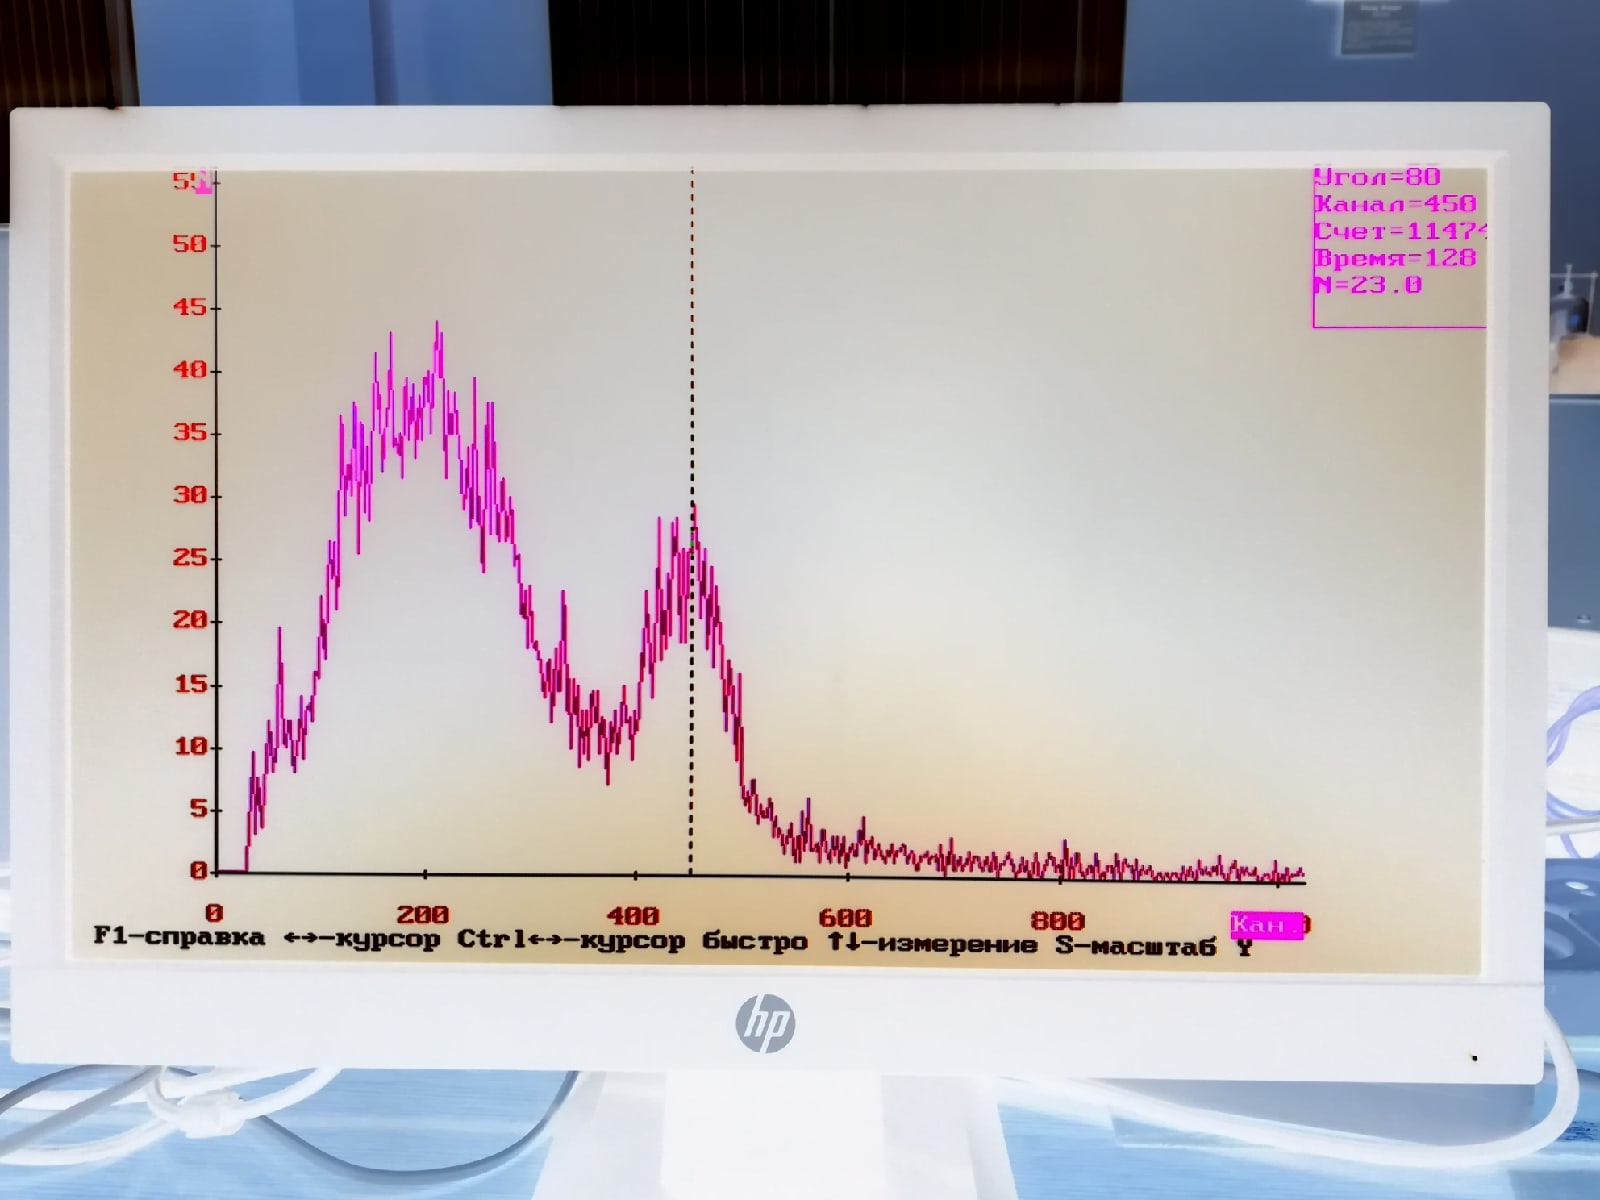
\includegraphics[width=\linewidth]{src/80Neg} \\ б)}
		\end{minipage}
		\caption{Распределения на экране компьютера: a) угол $\theta = 20^\circ$; б) угол $\theta = 80^\circ$}
	\end{figure}

	\begin{figure}[h!]
		\centering
		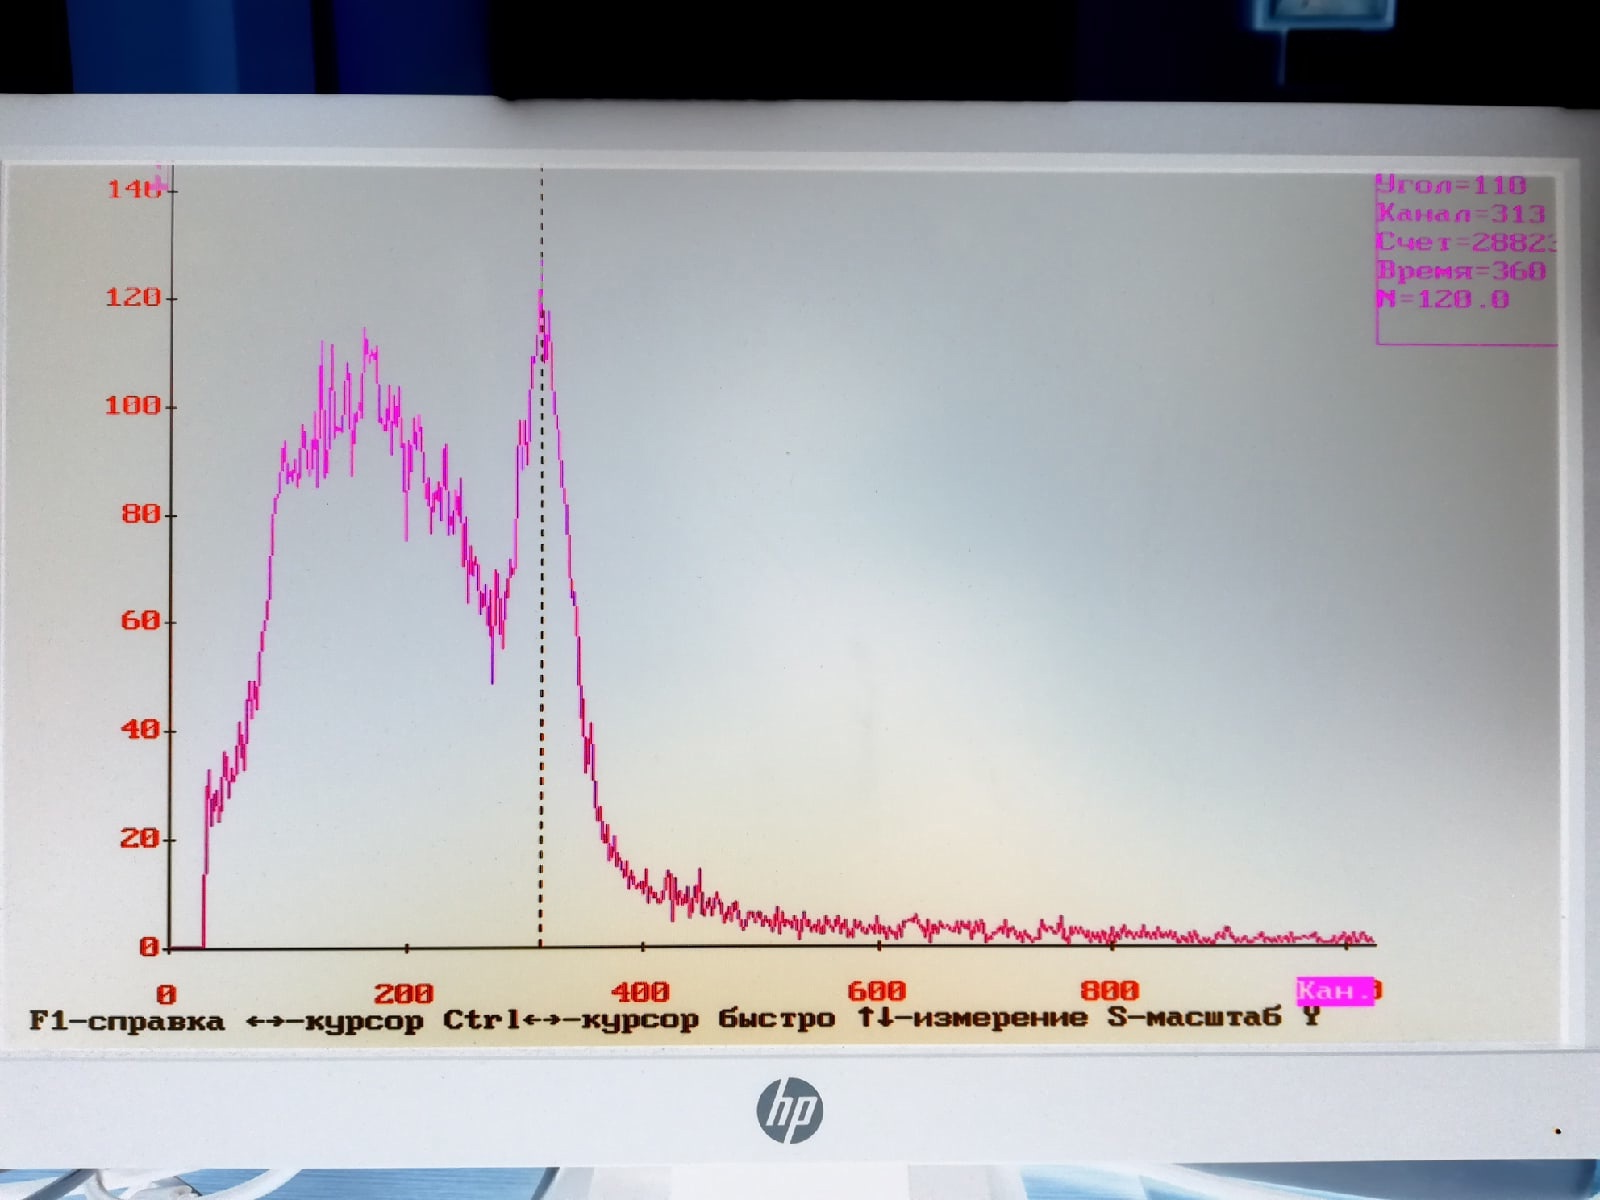
\includegraphics[width=\linewidth]{src/110Neg}
		\caption{Распределение на экране компьютера: угол $\theta = 110^\circ$}
	\end{figure}


 \begin{table}[h!]
		\centering
		\begin{tabular}{|c|c|c|c|c|c|c|c|c|c|c|c|c|c|}
			\hline
			$\theta^\circ$ & 0   & 10   & 20  & 30  & 40  & 50  & 60  & 70  & 80  & 90  & 100 & 110 & 120 \\ \hline
			$N$            & 900 & 1011 & 819 & 779 & 702 & 621 & 553 & 470 & 437 & 378 & 346 & 313 & 298 \\ \hline
			$\sigma_N$     & 10  & 11   & 9   & 8   & 8   & 7   & 6   & 5   & 5   & 4   & 4   & 4   & 3   \\ \hline
		\end{tabular}
		\caption{Зависимость номера канала $N$ от угла $\theta$}
		\label{Compton_Table}
	\end{table}

	Погрешность $\sigma_N$ складывается из погрешностей определения $N$ самого прибора $\sigma_N^\text{приб} = 0,01N$ и погрешности измерения по прибору $\sigma_N^\text{изм} = 1$. Суммарно: $\sigma_N = \sqrt{(\sigma_N^\text{приб})^2 + (\sigma_N^\text{изм})^2}$.
	
	
	Заменим в формуле \eqref{Energy_Compton} энергию квантов, испытавших комптоновское рассеяние на угол $\theta$, номером канала $N(\theta)$, соответствующего вершине фотопика при указанном угле $\theta$. Обозначая буквой $A$ неизвестный коэффициент пропорциональности между $\varepsilon(\theta)$ и $N(\theta)$, найдем:
	\begin{equation}
		\frac{1}{N(\theta)} - \frac{1}{N(0)} = A(1 - \cos\theta).
	\end{equation}
	
	Возвращаясь от переменной $\varepsilon$ к энергии $E$, мы получаем, что при $\theta = 90^\circ$ формула \eqref{Energy_Compton} принимает вид
	\begin{equation*}
		mc^2 \left(\frac{1}{E(90)} - \frac{1}{E(0)}\right) = 1,
	\end{equation*}
	\noindent или
	\begin{equation}
		mc^2 = E(0)\frac{E(90)}{E(0) - E(90)} = E_\gamma \frac{N(90)}{N(0) - N(90)}.
		\label{Compton_mc2}
	\end{equation}
	
	В этой формуле $E(0) = E_\gamma$ -- энергия электронов, рассеянных вперед, -- просто равна энергии $\gamma$-лучей, испускаемых источником.
	
	
	Используя экспериментальные результаты, построим график, откладывая по оси абсцисс величину $1 - \cos\theta$, по оси ординат --- $1 / N(\theta)$. Так как мы знаем ошибку $\sigma_N$ для каждого значения, будем использовать метод минимума $\chi^2$. Примем также во внимание, что изначально устройство было, возможно, не откалибровано, поэтому углы были не совсем точными. Подставим для каждого значения угла $\theta \longrightarrow \theta + \Delta \theta$ в косинус и проварьируем по $\Delta\theta$ так, чтобы точки лучше легли на прямую, то есть $\chi^2 \rightarrow \min$.
	
	
	В нашем случае получаем: $\Delta \theta = -0.28^\circ$.
	
	И значение $\chi^2 \simeq 161$ -- это говорит о том, что экспериментальные значения колеблются в пределах $\sim 3\sigma$ от истинного значения.
	
	\begin{figure}[h!]
		\centering
		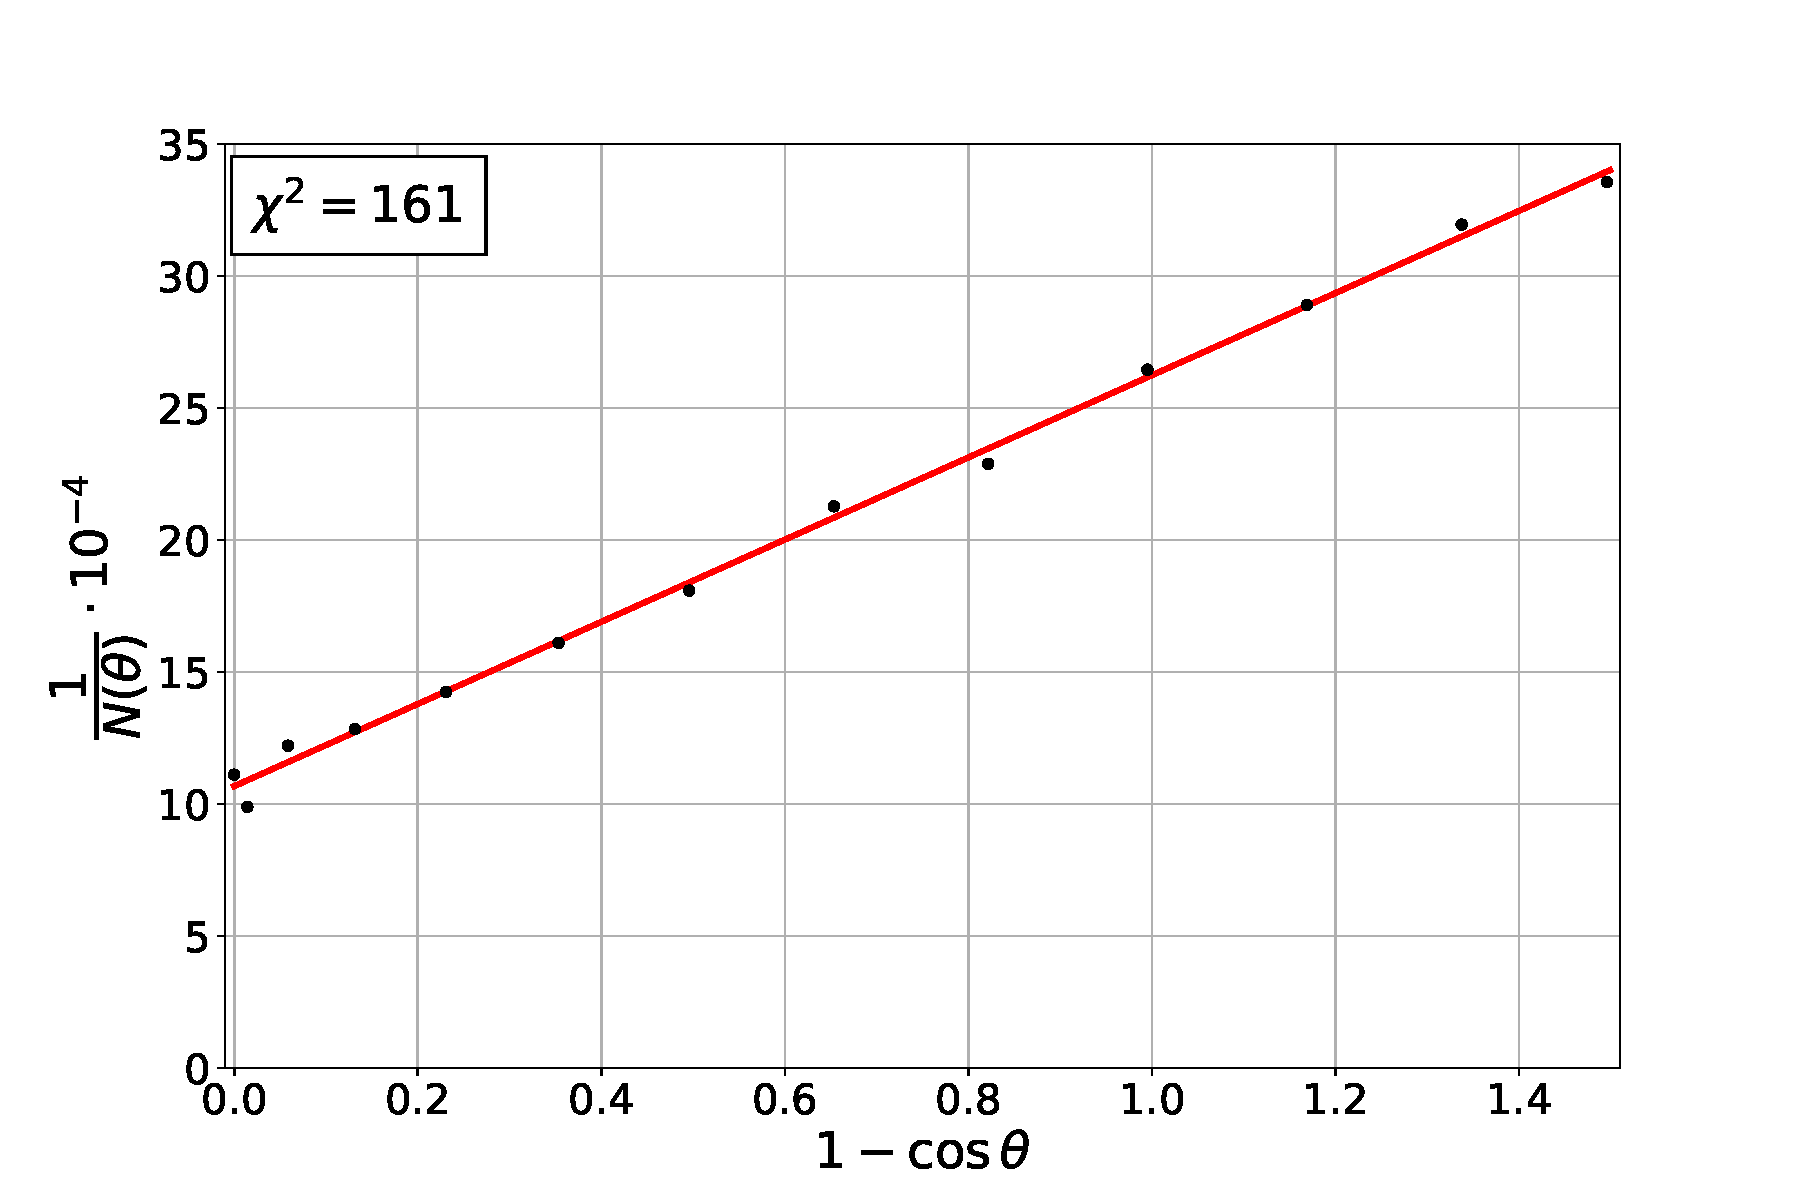
\includegraphics[width=\linewidth]{src/N(theta).pdf}
		\caption{Зависимость $\dfrac{1}{N(\theta)}$ от $1 - \cos \theta$}
	\end{figure}

	Из данного графика получаем следующие значения для наклона и пересечения с осью ординат соответственно:
	\begin{itemize}
		\item $k = (156 \pm 3) \cdot 10^{-5}$
		
		\item $b = (107 \pm 2) \cdot 10^{-5}$
	\end{itemize}
	
	Найдем $N(0)$. $N(0) = 1/b$

	Тогда получаем:
	\begin{equation*}
		\boxed{N(0) = (940 \pm 20)}
	\end{equation*}

	Найдем $N(90)$. Это значение $N$, при котором $\cos\theta = 0$. То есть, другими словами, $1 - \cos\theta = 1$. Тогда:
	\begin{equation*}
		N(90) = \frac{1}{k \cdot 1 + b} = \frac{1}{k + b}
	\end{equation*}

	В итоге находим:
	\begin{equation*}
		\boxed{N(90) = (380 \pm 10)}
	\end{equation*}

	
	Используя \eqref{Compton_mc2}, и то, что $E_\gamma = 662$ кэВ, найдем:
	\begin{equation*}
		\boxed{mc^2 = (450 \pm 20)\text{ кэВ}}
	\end{equation*}

	Как видно, данное значение имеет ошибку $\sim 5\%$. Табличное значение 511 кэВ, что, как и было сказано, укладывается в $\sim 3\sigma$.
	

    \clearpage
    
	\section*{Вывод}
 
    В работе мы исследовали эффект Комптона. Качественно пронаблюдали энергии рассеянных $\gamma$-квантов в зависимости от угла рассеяния. Также, была определена энергия покоя частиц, на которых происходит рассеяние (электронах): $mc^2 = (450 \pm 20)\text{ кэВ}$, что достаточно близко к табличному значению в 511 кэВ. Ошибка составляет порядка $5\%$.

    \vfill
    
    \begin{thebibliography}{9}
    	\bibitem{max} \emph{Лабораторный практикум по общей физике. В 3 томах. Том 3. Квантовая физика: учебное пособие} под ред. Ю. М. Ципенюка
    \end{thebibliography}

\end{document}
